\begin{table}[ht]
\centering\small
\caption{Stable-control decoded-operator rollout relative MSE, mean $\pm$ sample SD over three sampled systems. Calibration length is 128; lower is better. A zero-output predictor has error 1. Index bits exclude the stored FP32 radii; all compressed controls use identical bytes at each budget.}
\label{tab:memory}
\setlength{\tabcolsep}{3pt}
\begin{tabular}{lrrrr}
\toprule
& \multicolumn{2}{c}{4 index bits/mode} & \multicolumn{2}{c}{8 index bits/mode} \\
Method & $L=128$ & $L=512$ & $L=128$ & $L=512$ \\
\midrule
FP32 reference & $0.000\pm0.000$ & $0.000\pm0.000$ & $0.000\pm0.000$ & $0.000\pm0.000$ \\
Stable Cartesian weight & $1.137\pm0.185$ & $1.297\pm0.221$ & $0.841\pm0.022$ & $0.998\pm0.074$ \\
Stable Cartesian memory & $0.852\pm0.045$ & $0.936\pm0.031$ & $0.789\pm0.026$ & $0.922\pm0.027$ \\
Normalized Cartesian memory & $1.109\pm0.034$ & $1.308\pm0.070$ & $0.350\pm0.092$ & $0.998\pm0.177$ \\
Phase nearest & $1.503\pm0.188$ & $1.768\pm0.213$ & $0.117\pm0.024$ & $0.939\pm0.090$ \\
Phase weight & $1.612\pm0.109$ & $1.778\pm0.206$ & $0.094\pm0.031$ & $0.811\pm0.177$ \\
Phase memory & $0.967\pm0.074$ & $1.250\pm0.082$ & $0.094\pm0.033$ & $0.791\pm0.198$ \\
\bottomrule
\end{tabular}
\end{table}

\begin{figure}[ht]
\centering
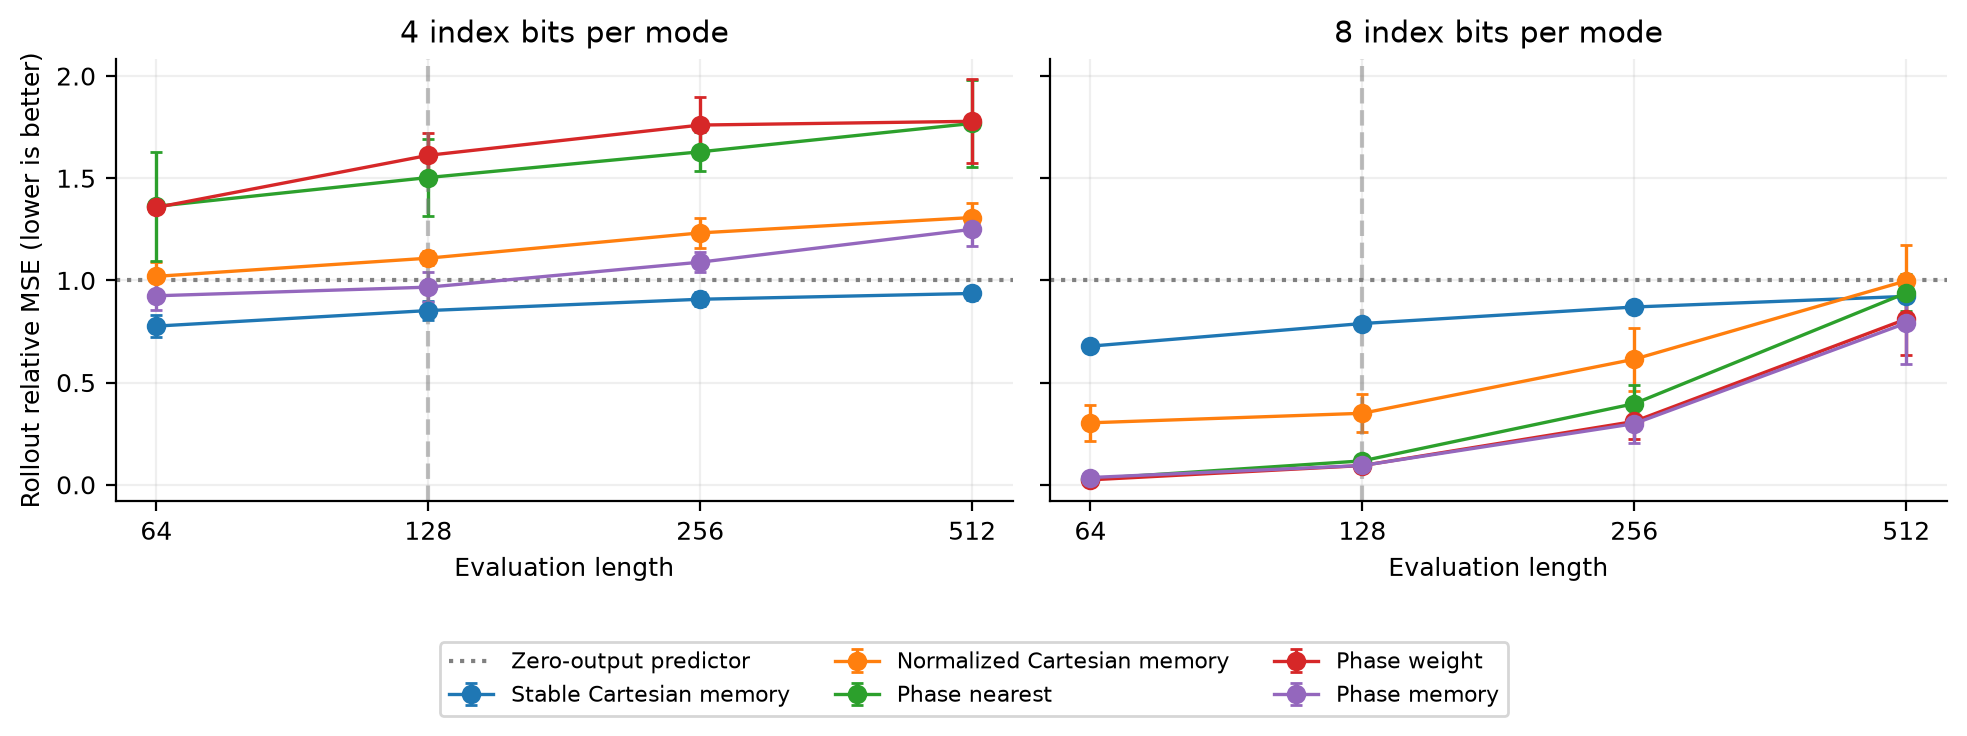
\includegraphics[width=\linewidth]{memory_comparison.png}
\caption{Stable-control comparisons over evaluation length. Error bars show sample standard deviation over systems. The dashed vertical line marks calibration length 128; the horizontal dotted line is a zero-output predictor.}
\end{figure}
The four-bit phase-memory control improves relative to phase-weight calibration, but the stable Cartesian memory control has lower mean error at length 512. Phase-memory relative error exceeds one at that horizon, indicating worse output reconstruction than predicting zero. The pilot therefore does not establish a useful long-context phase advantage. At eight index bits, phase-memory error at length 512 is approximately 0.791, compared with 0.811 for phase-weight calibration and 0.922 for stable Cartesian memory. The extra memory-objective improvement over phase-weight calibration is modest; only three systems are tested. The eight-bit setting is reported separately rather than pooled with the four-bit setting. The observed benefit of the memory objective within a representation must not be conflated with superiority of that representation.

The nearest Cartesian decoder can have radii above one and exhibits catastrophic growth. This diagnostic should not dominate the assessment: fitted Cartesian controls are explicitly stabilized, and the normalized Cartesian control provides a fixed-radius comparison. Reported sample deviations are descriptive over only three systems; no significance claim is justified. Version 1, with unconstrained fitted Cartesian controls and numerically unreliable large-error coordinate comparisons, is retained as a diagnostic. Version 2 uses stable initialization and constraints for fitted raw Cartesian controls and supplies all tabulated results.
